% \documentclass{beamer}
% \usetheme{Szeged}

% \begin{document}


%-------------------------------------------------------------------------------
%							FIRST SECTION
%-------------------------------------------------------------------------------

%------------ Intro Part 2
% - le site de l'IRMA est riche et complet
% - De M.NAVORET et FRANCK vers l'equipe MOCO (leurs travaux, etc..):
% - l'equipe probabilite

\section{Introduction}    % L'IRMA

\subsection{L'IRMA}
	
\begin{frame}
\frametitle{L'equipe MOCO}
% MM. Franck et Navoret
	Plusieurs membres parmi lesquels MM.: % M. Prud'homme aussi
	\begin{itemize}
		\item Emmanuel FRANCK % Dernier expose: Base de modèles épidémiologiques, covid et contrôle (2020)
		\item Laurent NAVORET % Dernier expose: Modèle macroscopique pour un système de particules discoïdales en interactions d'alignement (2015)
  \end{itemize}
  Responsables des seminaires en EDP

  \pause
  % L'equipe MOCO en general (analyse des EDP, de la théorie du contrôle, du calcul scientifique et haute performance, et des statistiques.)
	\begin{itemize}
		\item Partenariats internationaux (Portugal, Allemagne, USA, etc.)  % Projets (Examag Spexxa, MAToS, projet EUROFUSION)
		\item Partenariats indutriels  % 
		\item Modélisation des plasmas  % L’équipe projet INRIA TONUS qui lui est adossee
  \end{itemize}

\end{frame}

% \subsection{L'équipe Probabilités}
	
\begin{frame}
\frametitle{L'equipe Probabilites}
% MM. Franck et Navoret
	Plusieurs membres parmi lesquels M.: % M. Prud'homme aussi
	\begin{itemize}
		\item Vincent VIGON
  \end{itemize}

  \pause
  % L'equipe Probabilites en general
  Des activites diverses:
	\begin{itemize}
		\item Partenariats internationaux (Allemagne, Autralie, Chine, etc)  % Actuariat, Transport optimal, Matrrice Aleatoire
		\item Séminaire (de calcul) stochastique.  % 
  \end{itemize}

% You get the point, ce sint de grosses equipes de recherches tres actives! Et des que j'ai vu qu'elles allait encadrer le projet, j'ai saute sur l'occasion

\end{frame}

\subsection{Le sujet du stage}

\begin{frame}
  \frametitle{Le(s) problème(s) à résoudre}

\begin{columns}
 \begin{column}{0.5\textwidth}
  \centering
    Probleme direct \\ (\scriptsize Resolution de l'ETR par un schema de "splitting")
    % Image de densite -> signal sur les bords
      % 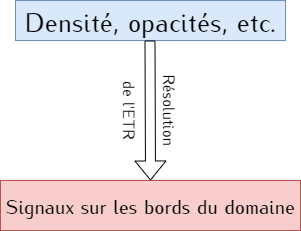
\includegraphics[width=5cm]{ProblemeDirect}       
  \end{column}
 \pause
 \begin{column}{0.5\textwidth}
    \centering
    Probleme inverse \\ (\scriptsize Reconstruction de la densite par un reseau de neurones)
    %Image de signal sur les bords -> densite
      % 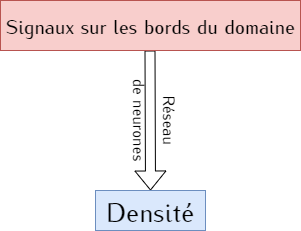
\includegraphics[width=5cm]{ProblemeInverse}       
 \end{column}
\end{columns}

\begin{figure}
  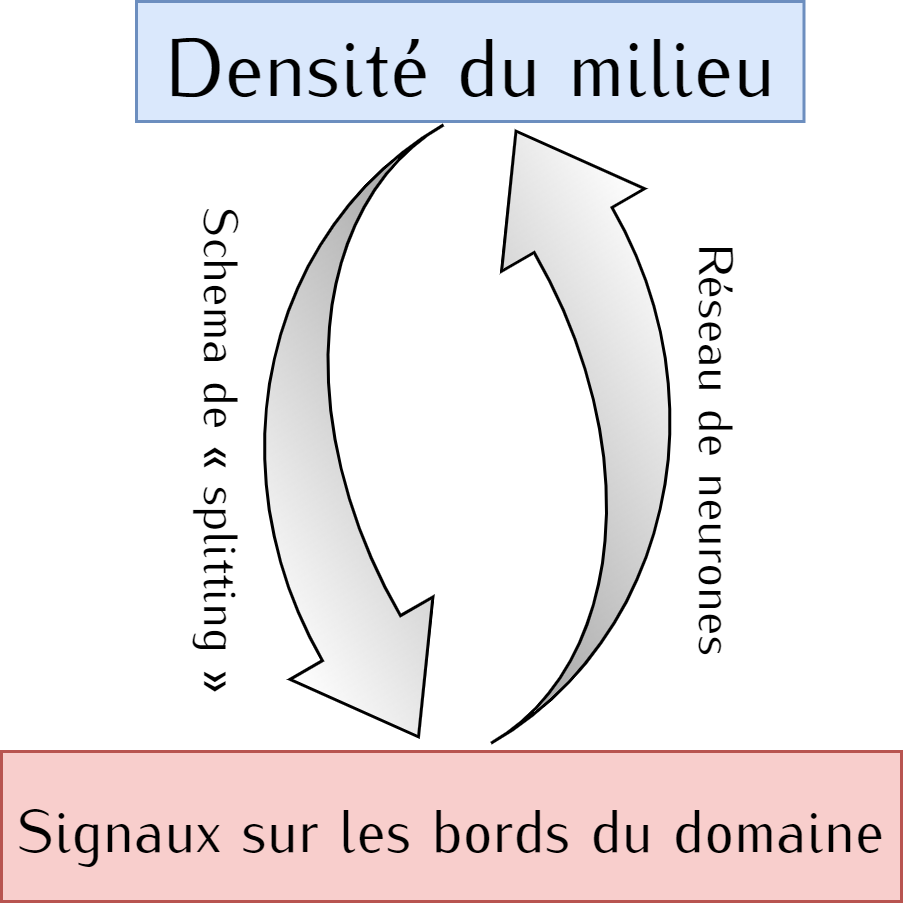
\includegraphics[width=4cm]{PBInverse}         
\end{figure}

\end{frame}
%-------- Vrai debut de l'introduction (PB INVERSE)
\begin{frame}
  \frametitle{Les point pour situer le stage}

  \begin{enumerate}
    \item Explosion du deep learning % Depuis le debut de la decenie 2010, le Machine Learning a considerablement pris de l’ampleur (2015 a l’ILSVRC, etc..)
    %%%%%% IMAGE DU DEEP LEARNING
    \item APplications dans le secteur medical (Imagerie medicale) % Avant de soigner les cancers, on doit detecter les tumeurs sont plus denses que les tissus sains (Chercher d'autres applications)
    %%%%%% IMAGE DU MEDICAL
    \item Reevaluation des methode de resolution de problemes inverse % Les problemes inverses sont difficiles. ... Les algo d'optimisation classiques marchent tres bien. En fait on s'est referer aux travaux de Maya et Guillaume Dolle. L'avantage que peuvent offrir les ANN c'est juste la simplicite, et la rapidite, et une generalisation (non specificite aux probleme)
    %%%%%% IMAGE DU PB INVERSE
  \end{enumerate}
  
\end{frame}

\begin{frame}
  \scriptsize
  \frametitle{Sommaire}
  \tableofcontents
\end{frame}


% \end{document}
